\subsubsection{Diferencia de frecuencias absolutas}
Como bien apuntan \cite{monroe2008fightin}, esta comparación no resulta tan rica
a la hora de contrastar lemas empleados por los distintos conjuntos de
votantes puesto que se ve fuertemente influenciada por la cantidad y longitud
de los discursos emitidos por cada grupo.
\par
En nuestro caso, se observa que la mayor\'ia de los lemas son característicos
del grupo de los votantes positivos, pero esto es una consecuencia del hecho
de que es el conjunto de estos votantes precisamente el que mayor cantidad de
discursos emitió, así como también, de mayor longitud, como muestra la distribución
de la figura \ref{fig-distrib-unique-tokens}. Asimismo, vemos en la figura
\ref{fig-statistics-freq-abs} que las palabras identificadas como características
de cada grupo (las azules, de los votantes a favor y las rojas, de los votantes
en contra) no resultan significativas puesto que la mayoría de ellas constituyen
palabras con escaso o nulo significado semántico (son verbos como `tener' o
determinantes, como `el' o `la'). Esto se evidencia sobre todo en el caso de
los votantes a favor.

\begin{figure}[h!]
    \centering
    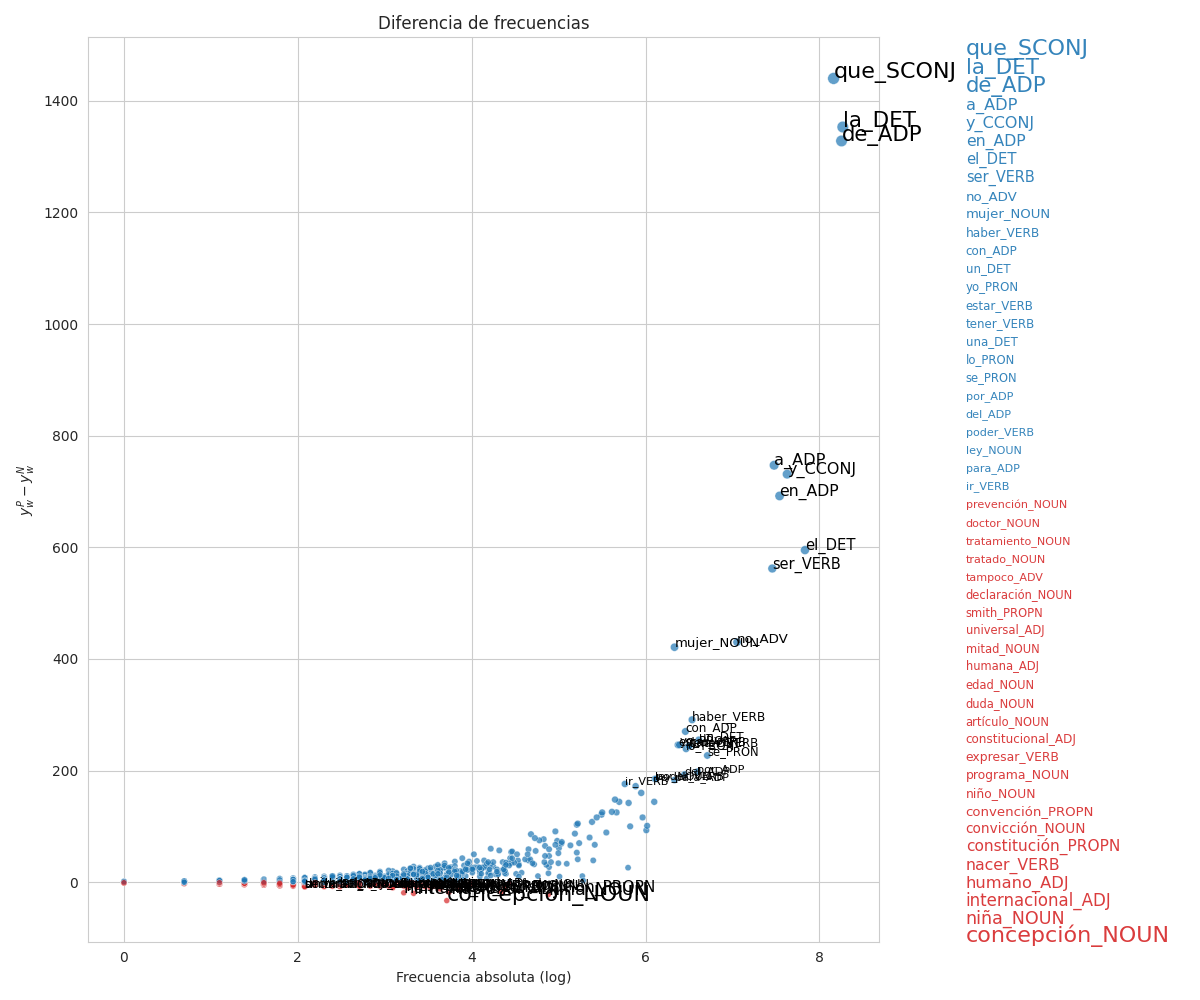
\includegraphics[scale=0.4]{../visualizations/stats/frecuencias.png}
    \caption{Comparación de palabras características de los votos afirmativos y
    negativos tomando como medida la diferencia de frecuencias absolutas descripta
    en la sección \ref{subsubsec-methods-freq-abs}. El eje de abscisas indica el
    logaritmo de la frecuencia absoluta de cada palabra en el conjunto de total
    de discursos y el eje de ordenadas, la comparación en cuestión. En la
    columna de la derecha se observan las 25 palabras más representativas de
    cada grupo de votantes escaladas según su relevancia.}
    \label{fig-statistics-freq-abs}
\end{figure}

Entre las 25 palabras más características del grupo de votantes positivos
encontramos mayormente determinantes (`la', `el', `un'), pronombres 
(`yo', `lo', `se'), preprocisiones (`de', `a', `en') o verbos de escaso
significado semántico (`ser', `haber', `estar'). La palabra más relevante
para la temática en cuestión parece ser el nombre `mujer', que denota a
quien, al menos desde cierta perspectiva, es el
sujeto protagonista en el curso de un embarazo y un posible aborto. En el grupo
de votantes, sin embargo, pueden observarse una mayor cantidad de palabras
de contenido que parecen reflejar cierta
postura o cuestionamiento respecto del aborto: sobre su consitucionalidad
y su lugar en la vida de una sociedad o privada de los ciudadanos
(`civil', `constitucional'), sobre si resulta un acto moral (`mala'),
sobre qué actos poner el foco (`respetar', `nacer', `concepción').

\subsubsection{Diferencia de proporciones}
\label{subsubsec-results-proporcions}
Al normalizar la frecuencia absoluta de cada palabra con la cantidad
de palabras totales emitidas por cada grupo, el cálculo de proporciones permite
superar la limitación observada en el apartado anterior.
La figura \ref{fig-statistics-proportions} ya no muestra en su mayoría palabras
vinculadas al grupo de votantes a favor de la legalización, sino que también
deja ver una gran cantidad de palabras relacionadas al grupo de votantes en contra.
Sembargo, este análisis sigue careciendo de validez semántica puesto que, como bien
indican \cite{monroe2008fightin}, no deja de asignarle mayor peso a aquellas palabras
que ocurren con más frecuencia. Si bien se observa una mayor presencia de palabras
con cierta significatividad para la temática abordada, la mayoría de los lemas
que el procedimiento arroja como característicos están más asociados a palabras
de uso frecuente en la lengua, más que a posiciones políticas particulares. Así,
dentro de las palabras indicadas como representativas de los votantes a favor,
volvemos a encontrar determinantes (`la', `esa'), preprocisiones (`a', `en'),
y adverbios (`hoy', `también'). Pero también se encuentran nombres y verbos
de relevancia que parecen indicarnos cuál es el centro de la discusión para el
grupo de votantes a favor de la legalización: la mujer, el embarazo y la
de decisión. Por parte del grupo de votantes negativos, similar al caso de
la diferencia de frecuencias absolutas, las palabras que resultan
características parecen resaltar  el momento de la concepción y el nacimiento.
También vuelve a aparecer cierta cuestión sobre lo consitucional o sobre el derecho.
E irrumpe, como novedad, la palabra `vida'.

\begin{figure}[h!]
    \centering
    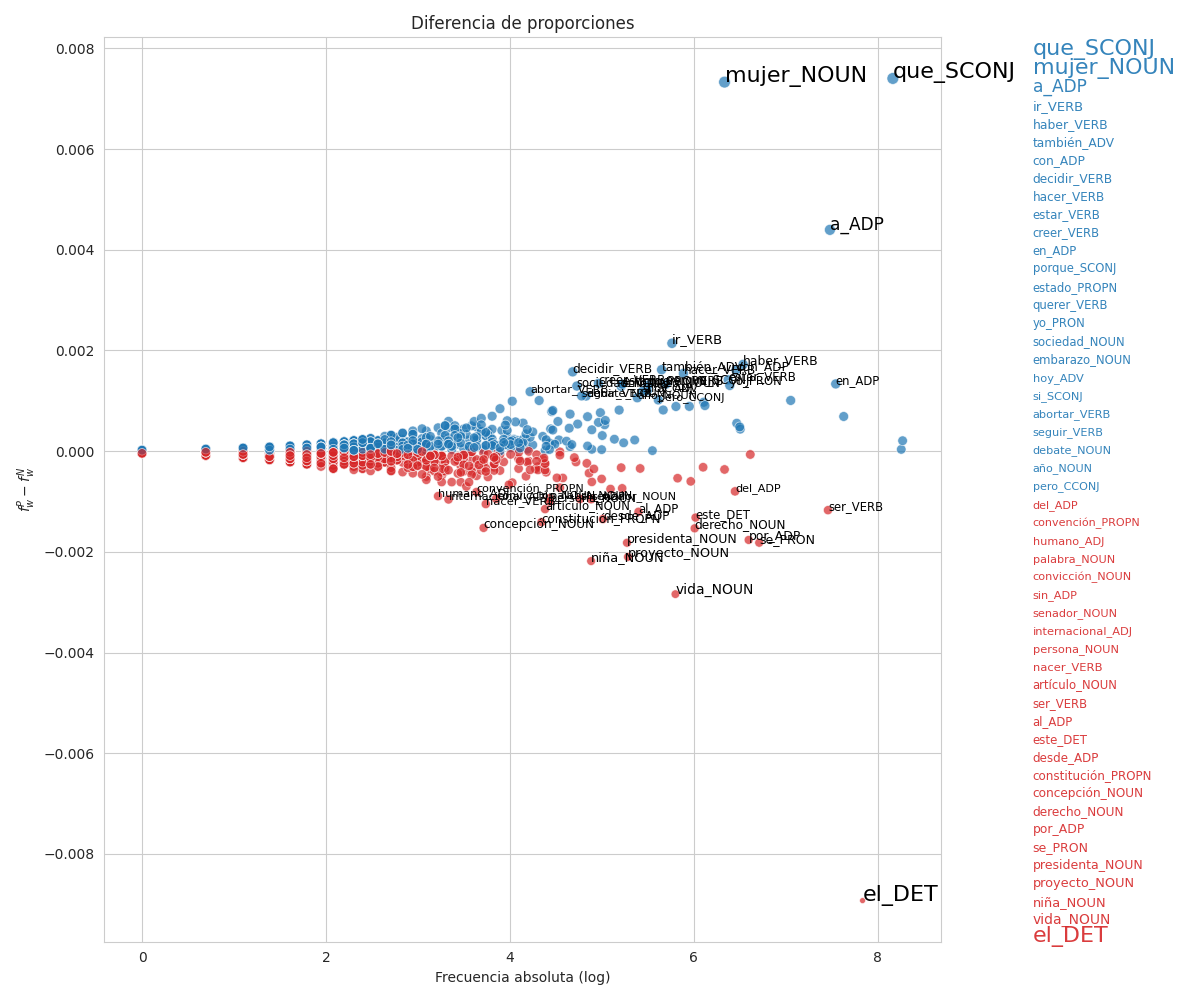
\includegraphics[scale=0.4]{../visualizations/stats/proporciones.png}
    \caption{Comparación de palabras características de los votos afirmativos y
    negativos tomando como medida la diferencia de proporciones descripta
    en la sección \ref{subsubsec-methods-proportions}.}
    \label{fig-statistics-proportions}
\end{figure}

\paragraph{Corrección: remoción de \textit{stopwords}}
\cite{monroe2008fightin} señalan que, si bien numerosos abordajes proponen remover
las palabras consideradas \textit{stopwords} del \textit{corpus} a analizar con el
fin de no viciar métricas como el cálculo de proporciones, ellos consideran inapropiado
emplear tales metodologías puesto que es posible que, en tal remoción, se acaben
eliminando también palabras de interés para el estudio en cuestión. En este caso,
palabras como `ella' podrían ser eliminadas cuando resultan sumamente relevantes
puesto que quienes atraviesan un embarazo y, potencialmente, la necesidad de un
aborto, son mujeres, por lo que la presencia de tales vocablos en el discurso, sumado
a otras palabras, puede indicar cierto posicionamiento. Con el objectivo de
contrastar lo sostenido por los autores, aquí se intentaron dos remociones empleando
distingos métodos para la definición del conjunto de \textit{stopwords}.

\subparagraph{Librería NLTK}
Como se adelantó en \ref{subsubsec-methods-proportions}, se tomó el conjunto cerrado de
\textit{stopwords} predefinido por esta librería y se removió tales ocurrencias
del corpus trabajado.
Luego se volvió a realizar el análisis de proporciones y, esta
vez, se observó una menor cantidad de palabras funcionales,
como preposiciones o determinantes, dado que suelen ser estas
las palabras catalogadas como \textit{stopwords} en la mayoría de
los \textit{corpora} prefefinidos. Y, una vez más, apreciamos palabras que indicarían
cierto foco del debate en la mujer, la decisión, la autonomía y la posibilidad de
interrupción. Emerge un nuevo concepto, como el de la clandestinidad, y también
el de gestante, que permite describir a la persona que atraviesa un embarazo por
su condición transitoria antes que por su identida de género o, incluso, su
sexualidad.
En cuanto a los discursos que se pronunciaron en contra, volvemos a
encontrar una fuerte presencia de lemas vinculados al deber, el derecho
el respeto, entre otros que parecen referir al marco legal que rige una
sociedad. Del mismo modo, se vuelven a hallar como temáticas el nacimiento,
la concepción y la vida.

\subparagraph{Ley se Zipf}
Para la selección de \textit{stopwords} utilizando el análisis de la Ley de Zipf,
se ordenaron las palabras según su frecuencia de manera decreciente y se estableció
un umbral: las palabras ubicadas por encima de este umbral en el \textit{ranking}
se consideraron \textit{stopwords} debido a consituyen palabras de uso más
frecunete en el \textit{corpur} y, por tal motivo, fueron removidas.
Esto llevó a la remoción de las primeras cien palabras más frecuentes, entre 
las cuales, la mayoría forma parte de palabras funcionales.
Los pocos casos que no responden a esta característica son palabras pasibles de
ser consideradas de uso frecuente en el género discursivo propio del debate político
y de esta temática en cuestión, como `aborto' y `vida'.
En el apéndice \ref{appendix-plots-zipf-law} podemos ver el gráfico que contrasta
las frecuencias de las palabras y su orden en el \textit{ranking}.
Luego de extraer el conjunto de palabras seleccionado, se procedió a realizar el
mismo análisis de proporciones detallado en este apartado. Nuevamente, entre
los discursos a favor, se observaron palabras relacionadas con la decisión, aunque
esta vez aparecieron nuevos términos, como `voluntaria', `elegir'. Se hace presente
también la cuestión de la regulación (`legal', `justicia', `clandestinidad') y
surgen nuevos términos como `ella', `morir', `cuerpo', `igualdad'.\todo{esto se retoma después?}
Por parte de los discursos en contra, volvemos a encontrar vocablos relacionados
con la normatividad (`constitucional', `código', `convención', `cumplir', 
`acuerdo', `tratado') y, una vez más, se presentan términos relacionados
con la concepción y el nacimiento.

\begin{figure}[h!]
    \centering
    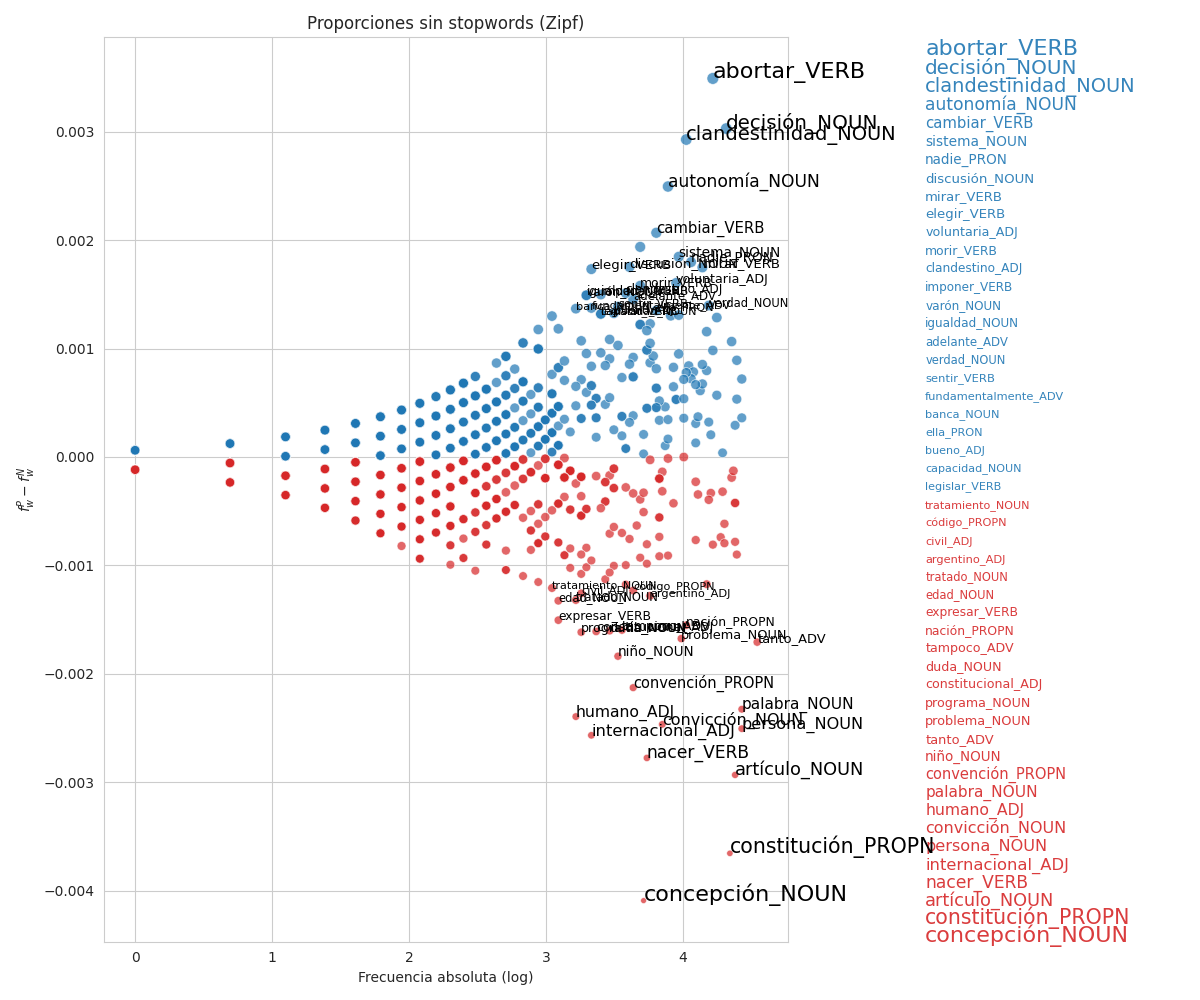
\includegraphics[scale=0.4]{../visualizations/stats/proporciones_sin_stopwords_zipf.png}
    \caption{Comparación de palabras características de los votos afirmativos y
    negativos tomando como medida la diferencia de proporciones descripta
    en la sección \ref{subsubsec-methods-proportions} luego de la remoción de
    \textit{stopwrods} utilizando la Ley de Zipf.}
    \label{fig-statistics-proportions-zipf}
\end{figure}

\subsubsection{Ratio de \textit{Odds}}
A diferencia de los casos anteriores, por la definición de la función de
\textit{ratio} de \textit{odds}, el punto de corte para considerar
a una palabra como característica de cada discurso ya no es el $0$ sino el $1$:
las palabras por encima de ese umbral serán las positivas y aquellas por debajo,
las negativas. Nótese que, dado que la ocurrencia de una palabra nunca es negativa,
los \textit{ratios} calculados solo arrojarán valores positivos. Por otro lado,
la función no estará definida para los casos en los cuales una palabra se
observe solamente en el conjunto de discursos a favor, dado que no es posible
dividir por $0$. Se observaron 1871 registros en esta situación, todos ellos
pertenecientes a palabras presentes en los dicursos positivos y ausentes En
los negativos.
\par
Al analizar las palabras arrojadas como representativas de cada discurso, se
encuentra que el grupo de votantes a favor hace referencia a las violaciones
(con el adjetivo `violada'); a la clandestinidad (con el adjetivo `clandestina'),
y a la interrupción legal del embarazo (con la sigla `ILE'). Vuelve a aparecer,
a su vez, la cuestión de la elección (con el verbo `elegir'), y hallamos también
la presencia de verbos referentes al castigo (`castigar'), al parto (`parir') y
al hecho de juzgar. Por otro lado, en los discursos negativos se encontraron
adjetivos como `inoportuno'; sustantivos como `respaldo', `juicio' y `hambre', 
y verbos como `aprovechar' y `justificar'.

\subsubsection{Ratio \textit{Log-odds}}

Los resultados de aplicar el logaritmo sobre el ratio de \textit{odds} no distaron
de los observados sin su aplicación. La única mejora se dio en
términos de la visualización de los datos: al tomar logaritmo, el umbral que separa
las palabras de los discursos positivos de los negativos vuelve a ser el $0$ y,
similar a lo que ocurre en los gráficos anteriores, los puntos representativos
de las palabras se ordenan de forma espejada, mientras que, sin tomar logaritmo,
esto no ocurrió y la interpretabilidad de los datos resultó más dificultosa.

\paragraph{Suavizado}
Así como ocurría con el ratio de \textit{odds}, el ratio de \textit{log-odds} no
permite capturar claramente aquellos csos en los que una palabra solo se observa en
un grupo de discursos pero no en el otro. Por su formulación, cuando una palabra
ocurra solamente en los discursos negativos, el logaritmo devolverá el valor $1$ y,
cuando solo ocurra en los discursos positivos, la función estará indefinida. Para
superar esta limitación, se aplicó un suavizado sobre tales casos.
\par
Sin embargo, como señalan \cite{monroe2008fightin}, si bien esta técnica permite
lidiar con las palabras conf frecuencia $0$ para algún grupo discursivo, arroja,
en cada caso, un conjunto de palabras cuya interepreación resulta un poco más
oscura respecto de la su relevancia para el tópico en cuestion. En el caso
de los discursos a favor, podemos encontrar algunas más claras como `médica',
`matriculado', `privilegiado', entre los adjetivos, y `solvencia', entre los nombres,
pero otras menos claras como `operatividad', `tapita', `alcohol', `postre',
`desencuentro'. Y, por parte de los discursos en contra, vemos `dramáticp', `sordo' y
`biológico', como casos de adejtivos que podrían ser más fácilmente vinculados a la
temática, y `horizontal', `restringida', `pavada', `plasmada', `transitado', `sumado',
`ilustrar', como casos que, al menos, requieren un análisis más agudo para poder
aventurar una interepreación.

\subsubsection{\textit{TF-IDF}}

\paragraph{Frecuencia de documentos natural}
Similar a lo hallado por \cite{monroe2008fightin}, esta métrica presenta una
fuerte correlación ($-0.96$) con los resultados arrojados por la diferencia
de proporciones. La misma es de tipo inverso debido a la naturaleza del cálculo
utilizado: la frecuencia relativa es simpre positiva y el logaritmo de la
frecuencia inversa de un término en los documetnos, negativo. De modo que aquí,
a diferencia de los gráfios anteriores, los lemas representativos de los discursos
a favor se visualizarán debajo del eje `x' y aquellos representativos de los
discursos en contra, por encima. Quitando esta salvedad, las palabras observadas
para cada grupo son las mismas que las detalladas en la sección
\ref{subsubsec-results-proporcions} para la diferencia de proporciones.

\paragraph{Frecuencia de documentos con logaritmo}
Esta métrica no mostró resultados de fácil interpretación. Las palabras de cada
grupo resultaron ampliamente variadas y con poca conexión semántica
entre sí y con la temática de interés. Es por esto que, por cuestiones de espacio,
omitiremos detallarla.

\subsubsection{\textit{Word Scores}}

--- POS
`a', `en', `con' (adp)
`hoy', `también' (adv)
`pero' (cconj)
`la', `esa', `su' (det)
`mujer', `aborto', `embarazo', `sociedad', `debate', `año', `decisión', `clandestinidad' (noun)
`yo' (pron)
`que' (sconj)
`decidir', `querer', `abortar', `haber', `seguir', `ir' (verb)
--- NEG
`internacional' (adj)
`desde', `al', `por' (adp)
`no' (adv)
`o' (cconj)
`el' (det)
`problema', `persona', `senador', `artículo', `concepción', `proyecto', `presidenta', `derecho', `niña', `vida' (noun)
`él', `esto', `se' (pron)
`constitución' (propn)
`tener', `nacer', `decir', `ser' (verb)

\begin{figure}[h!]
    \centering
    \includegraphics[scale=0.4]{../visualizations/stats/wordscores.png}
    \caption{Comparación de palabras características de los votos afirmativos y
    negativos tomando como medida el \textit{word score} descripto
    en la sección \ref{subsubsec-methods-wordscores}.}
    \label{fig-statistics-wordscores}
\end{figure}
